\chapter{Background}
\label{background}

\section{RoboCup Competition}
RoboCup is an international robotics competition founded in 1997. The aim is to promote robotics and AI research, by offering a publicly appealing, but formidable challenge. The name RoboCup is a contraction of the competition's full name, "Robot Soccer World Cup". The official goal of the project: ''By mid-21st century, a team of fully autonomous humanoid robot soccer players shall win the soccer game, complying with the official rule of the FIFA, against the winner of the most recent World Cup.'' Something that may seem impossible with today's technology. I would say that a more realistic goal is to make a team of robots playing soccer like humans and not better than them.

\section{RoboCup Soccer}
The main focus of the RoboCup competitions is the game of football/soccer, where the research goals concern cooperative multi-robot and multi-agent systems in dynamic adversarial environments. All robots in this league are fully autonomous. A competition which gives the possibility of doing research in a more entertaining way.
\paragraph{Humanoid}
In the Humanoid League, autonomous robots with a human-like body plan and human-like senses play soccer against each other. Dynamic walking, running, and kicking the ball while maintaining balance, visual perception of the ball, other players, and the field, self-localization, and team play are among the many research issues investigated in the league. 

\paragraph{Middle Size}
Middle-sized robots of no more than 50 cm diameter play soccer in teams of up to 6 robots with regular size FIFA soccer ball on a field similar to a scaled human soccer field. All sensors are on-board. Robots can use wireless networking to communicate. The research focus is on full autonomy and cooperation at plan and perception levels.
\begin{figure}[htb!]
\centering
  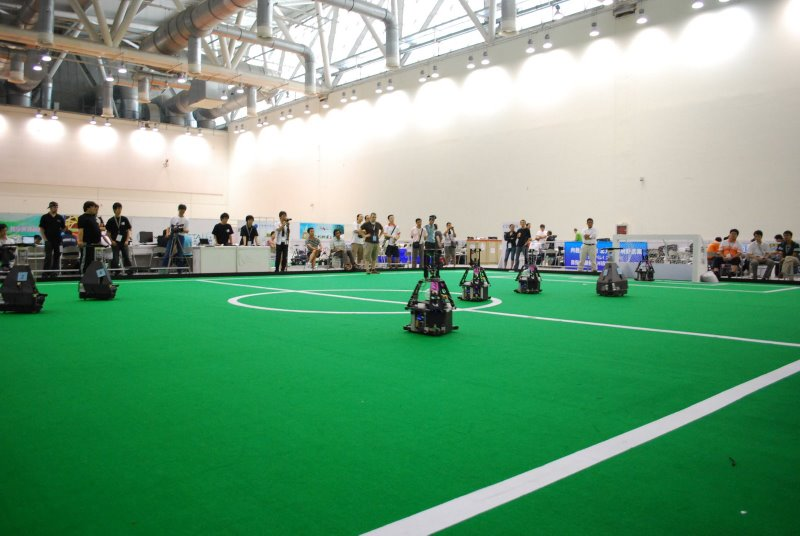
\includegraphics[width=0.8\textwidth]{Chapter1/figures/middleSize1.jpg}
  \caption{Middle Size League.}
  \label{fig:Middle}
\end{figure}
\paragraph{Simulation}
This is one of the oldest leagues in RoboCup's Soccer. The Simulation League focus on artificial intelligence and team strategy. Independently moving software players (agents) play soccer on a virtual field inside a computer. There are 2 subleagues: 2D and 3D. Simulation league 3D is going to be presented extensively in the next chapter. Figure \ref{fig:2d} shows how the 2D simulation league looks like.
\begin{figure}[htb!]
\centering
  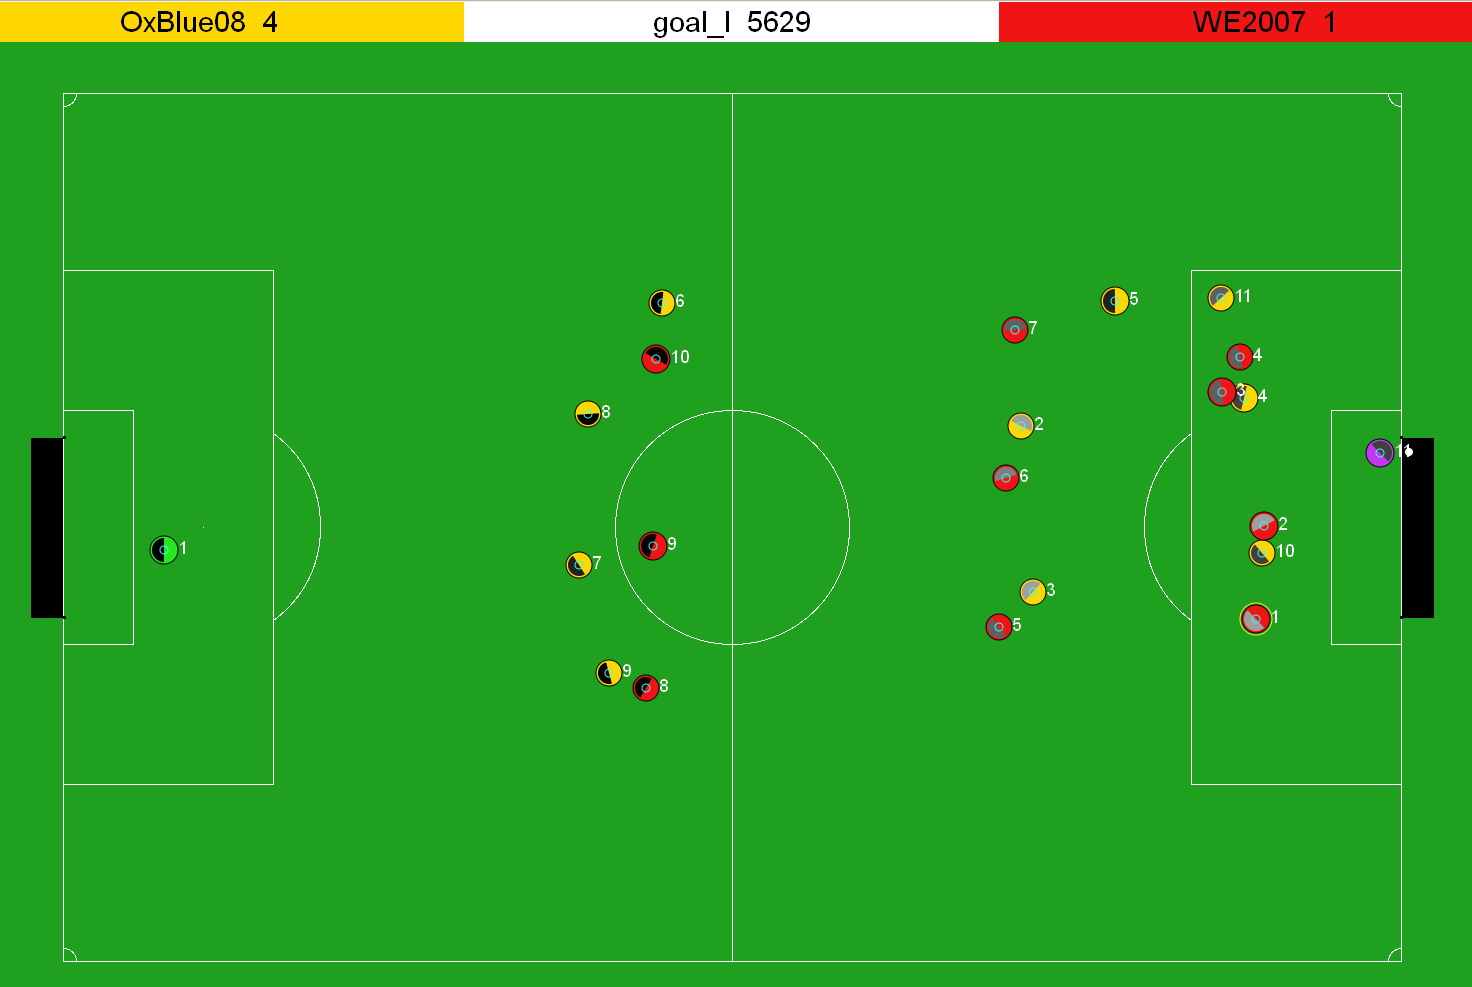
\includegraphics[width=0.8\textwidth]{Chapter1/figures/2D.jpg}
  \caption{2D simulation game.}
  \label{fig:2d}
\end{figure}
\paragraph{Small Size}
The Small Size league or F180 league as it is otherwise known, is one of the oldest RoboCup Soccer leagues. It focuses on the problem of intelligent multi-robot/agent cooperation and control in a highly dynamic environment with a hybrid centralized/distributed system.
\paragraph{Standard Platform}
In this league all teams use same robots. Therefore the teams concentrate on software development only, while still using state-of-the-art robots. Omnidirectional vision is not allowed, forcing decision-making to trade vision resources for self-localization and ball localization. The league is based on Aldebaran�s Nao humanoids. ''Kouretes'' from Technical University of Crete is the only Greek representative in this league, having continuous participations and lots of discriminations.
\begin{figure}[htb!]
\centering
  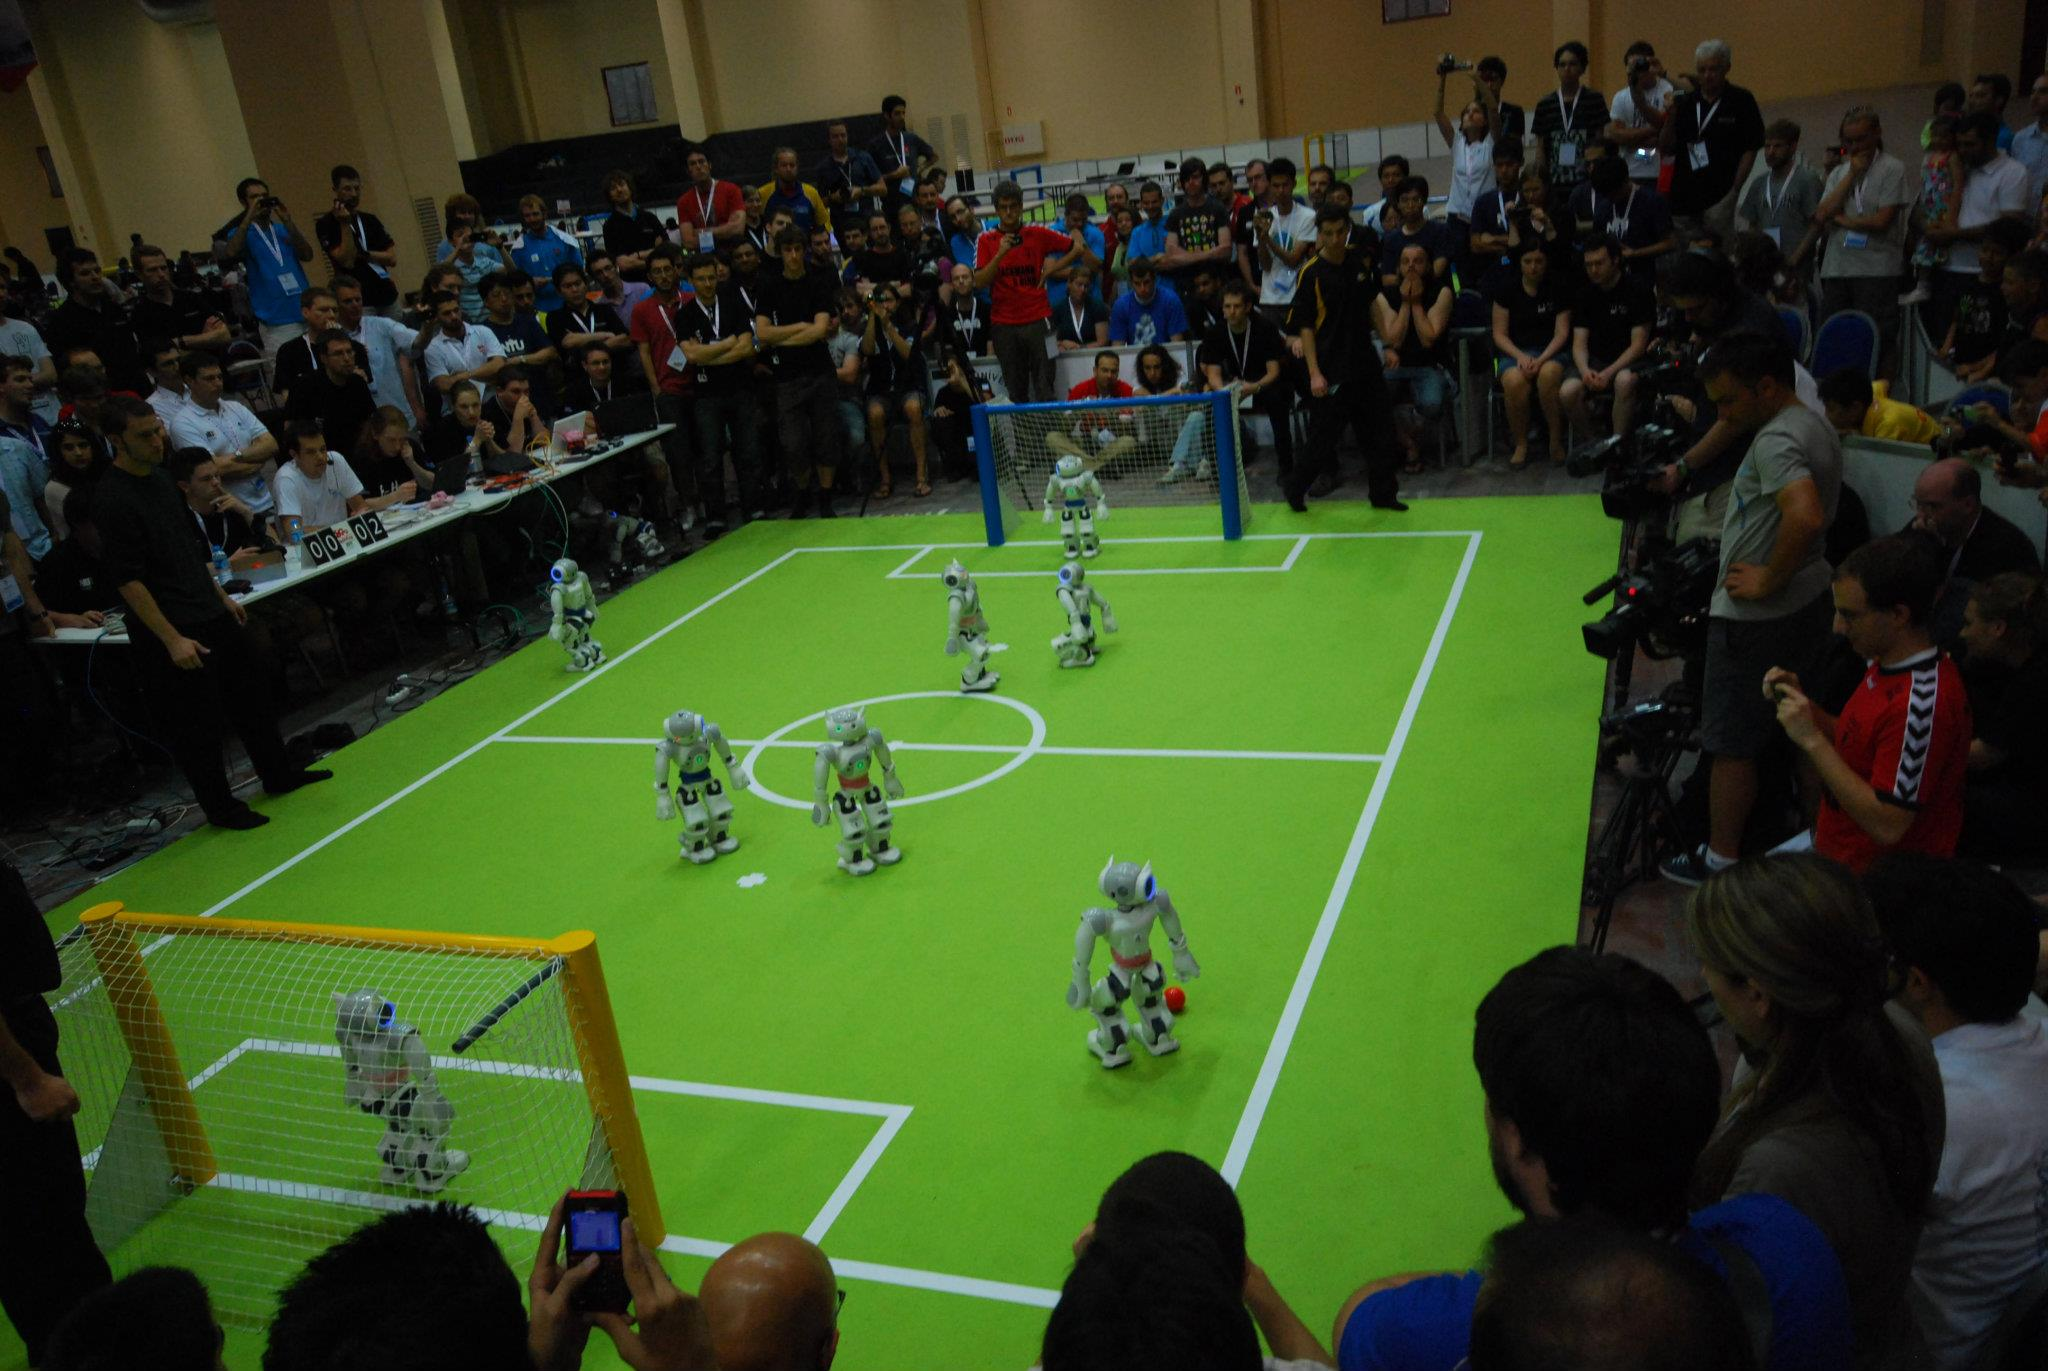
\includegraphics[width=0.8\textwidth]{Chapter1/figures/kouretes.jpg}
  \caption{Kouretes in action.}
  \label{fig:SPL}
\end{figure}
\section{RoboCup Rescue}
\paragraph{Robot League}
The goal of the urban search and rescue (USAR) robot competitions is to increase awareness of the challenges involved in search and rescue applications, provide objective evaluation of robotic implementations in representative environments, and promote collaboration between researchers. It requires robots to demonstrate their capabilities in mobility, sensory perception, planning, mapping, and practical operator interfaces, while searching for simulated victims in unstructured environments.
Greece has also a participation (2009) in this league by the Aristotle University's team called ''P.A.N.D.O.R.A''.
\begin{figure}[htb!]
\centering
  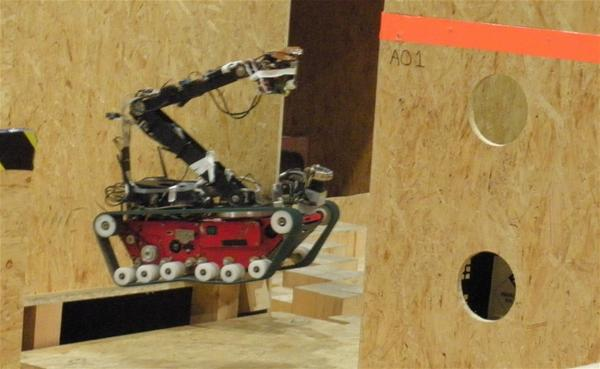
\includegraphics[width=0.8\textwidth]{Chapter1/figures/PANDORA.jpg}
  \caption{``PANDORA''.}
  \label{fig:pandora}
\end{figure}
\paragraph{Simulation League}
The purpose of the RoboCup Rescue Simulation league is twofold. First, it aims to develop develop simulators that form the infrastructure of the simulation system and emulate realistic phenomena predominant in disasters. Second, it aims to develop intelligent agents and robots that are given the capabilities of the main actors in a disaster response scenario.
\section{RoboCup @Home}
The RoboCup @Home league aims to develop service and assistive robot technology with high relevance for future personal domestic applications. It is the largest international annual competition for autonomous service robots and is part of the RoboCup initiative. A set of benchmark tests is used to evaluate the robots� abilities and performance in a realistic non-standardized home environment setting. Focus lies on the following domains but is not limited to: Human-Robot-Interaction and Cooperation, Navigation and Mapping in dynamic environments, Computer Vision and Object Recognition under natural light conditions, Object Manipulation, Adaptive Behaviors, Behavior Integration, Ambient Intelligence, Standardization and System Integration.
\begin{figure}[htb!]
\centering
  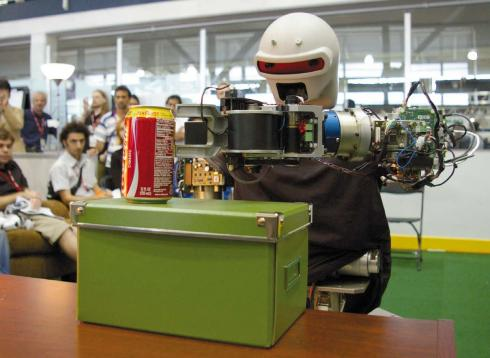
\includegraphics[scale=0.7]{Chapter1/figures/robocup@home.jpeg}
  \caption{RoboCup @Home.}
  \label{fig:RoboCup@Home}
\end{figure}
\section{RoboCup Junior}
RoboCupJunior is a project-oriented educational initiative that sponsors local, regional and international robotic events for young students. It is designed to introduce RoboCup to primary and secondary school children, as well as undergraduates who do not have the resources to get involved in the senior leagues yet. 
\paragraph{Soccer}
2-on-2 teams of autonomous mobile robots play in a highly dynamic environment, tracking a special light-emitting ball in an enclosed, landmarked field.
\paragraph{Dance}
One or more robots come together with music, dressed in costume and moving in creative harmony.
\paragraph{Rescue}
Robots identify victims within re-created disaster scenarios, varying in complexity from line-following on a flat surface to negotiating paths through obstacles on uneven terrain.